\documentclass[11pt]{amsart}
\usepackage{geometry}                % See geometry.pdf to learn the layout options. There are lots.
\geometry{letterpaper}                   % ... or a4paper or a5paper or ... 
%\geometry{landscape}                % Activate for for rotated page geometry
%\usepackage[parfill]{parskip}    % Activate to begin paragraphs with an empty line rather than an indent
\usepackage{graphicx}
\usepackage{amssymb}
\usepackage{epstopdf}
\usepackage{color}
\usepackage{amsmath}
\DeclareGraphicsRule{.tif}{png}{.png}{`convert #1 `dirname #1`/`basename #1 .tif`.png}

\title{Similarity solution for the case with a vegetation}
\author{Julia Lee}
%\date{}                                           % Activate to display a given date or no date

\begin{document}
\maketitle
\section{Governing Equation}
\subsection{Outside the vegetation}
\begin{equation}
u_x+v_y = 0
\end{equation}
\begin{equation}
uu_x+vu_y = -P_x/\rho + \nu (u_{xx} + u_{yy})
\end{equation}
\begin{equation}
uv_x+vv_y = -P_y/\rho + \nu (v_{xx} + v_{yy})
\end{equation}

\paragraph{\\Outside the vegetation, the flow behaves very closely similar to the flow above a flat plate with a free stream. Here, we assume the flow to be steady, incompressible, and laminar with constant fluid properties. Viscous dissipation is negligible in x-direction, and pressure is constant. Thus, we can use the Blasius similarity solution, where above equation reduces to :\\}

\begin{align}
u_x+v_y & = 0 \\
uu_x+vu_y &= \nu u_{yy} \\
P_y/\rho & = 0
\end{align}
\paragraph{ \\With Boundary Conditions\\}
\begin{equation}
u=0, v=0\; at\; y=0
\end{equation}
\begin{equation}
u \rightarrow U\; as\; y \rightarrow \infty
\end{equation}
\subsection{Inside the vegetation}
\paragraph{ \\Inside the vegetation, the momentum equation involves a drag term due to the drag exerted from the vegetation.\\}
\begin{equation}
uu_x+vu_y = -P_x/\rho -Du^2+ \nu (u_{xx} + u_{yy}) 
\end{equation}
\paragraph{\\The pressure inside the grass should match the pressure outside the grass in the boundary layer. And we know from outside of the vegetation, the Pressure gradients in both x and y goes to 0, thus here as well, \(Px \rightarrow 0\). Now we have\\}
\begin{equation}
uu_x+vu_y = -Du^2+ \nu (u_{xx} + u_{yy}) 
\label{inside_NS}
\end{equation}
\paragraph{ Let \(Ug \sim \) scale of the velocity near the tip inside the grass(deep inside the grass, the velocity goes to zero). Similarly, \(x \sim x\), \(y \sim \delta_I \), \(D \sim D\), and \(\nu \sim \nu \). Then the scales for each term in x-momentum equation are as follows:\\ }
\begin{gather}
uu_x+vu_y =  -Du^2+ \nu (u_{xx} + u_{yy})  \nonumber \\
\frac{Ug^2}{x}\quad \frac{Ug^2}{x}\quad DUg^2 \quad \frac{\nu Ug}{x^2} \quad \frac{\nu Ug}{\delta_I ^2} \nonumber
\end{gather}
\paragraph{ \\Comparing the third term with the fifth term;\\}
\begin{gather}
DUg^2 \quad \sim \quad \frac{\nu Ug}{\delta_I ^2} \nonumber \\
\delta_I = \sqrt{\frac{\nu}{UgD}} \quad \text{or} \quad Ug=\frac{\nu}{D\delta_I^2} \nonumber
\end{gather}
\paragraph{ \\Because at the boundary, \(u_{y}\) should be continuous; \(u_{y-} = u_{y+} \) \\}
\begin{gather}
\frac{\nu}{D \delta_I ^3}=\sqrt{\frac{U_\infty^3}{\nu x}}  \nonumber \\
\delta_I =D^\frac{-1}{3}\sqrt{\frac{\nu}{U_\infty} }x^\frac{1}{6}= \sqrt{\frac{\nu x}{U_\infty}} \frac{1}{(DX)^\frac{1}{3}}  \nonumber
\end{gather}
\paragraph{ \\Putting back \(\delta_I\) into the equation for \(Ug\) to check if \(Ug \ll U_\infty \) is satisfied.\\}
\begin{gather}
Ug \quad \sim \quad \frac{\nu}{D\delta_I ^2} \nonumber \\
\qquad \qquad \qquad \sim \quad \frac{\nu}{DD^\frac{-2}{3}\frac{\nu}{U_\infty}x^\frac{1}{3} }\nonumber \\
\qquad \qquad \sim \quad \frac{U_\infty}{(DX)^\frac{1}{3}}\nonumber
\end{gather}
\paragraph{\\ For \(Ug\) to go to 0, \(DX \gg 1\)}
\paragraph{\\Putting back \(Ug\) to the first, third and fourth term and compare to eliminate small terms. Here, the first two terms and the third and the fifth terms are of same scale, thus only one of each is compared: \\}
\begin{gather}
uu_{x}\; \text{;} \; \frac{Ug^2}{x} = \frac{U_\infty^2}{(DX)^\frac{2}{3}}\frac{1}{x}  \\
Du^2\; \text{;} \; \frac{U_\infty^2}{(DX)^\frac{2}{3}}D   \\
\nu u_{xx} \; \text{;} \; \frac{\nu Ug}{x^2} = \frac{\nu}{x^2} \frac{U_\infty}{(DX)^\frac{1}{3}} = \frac{\nu U_\infty}{D^\frac{1}{3}x^\frac{7}{3}}
\end{gather}
%DUg^2 = D \frac{U_\infty}{D^\frac{2}{3} x^\frac{2}{3}} \nonumber \\
%DX \gg 1 \nonumber
\section{Similarity solution}
\subsection{Outside the vegetation}
\begin{gather}
\eta = \frac{y}{\delta_O}, \qquad \delta_O = \sqrt{\frac{\nu x}{U_\infty}} \nonumber \\
f(\eta) = \frac{\Psi}{U_\infty \delta_O} \nonumber
\end{gather}
\begin{gather}
2f''' + ff'' = 0 \\
f'(0) = f(0) = 0, \qquad f'(\eta \rightarrow \infty) = 1
\end{gather}
\subsection{Inside the vegetation} 
\paragraph{From} 
\begin{gather}
0 = -P_x/ \rho -Du^2+ \nu u_{yy} \\
0 = -Du^2+ \nu u_{yy} \\
\eta = \frac{y}{\delta_I}, \qquad \delta_I = \sqrt{\frac{\nu}{U_\infty}} \frac{x^\frac{1}{6}}{D^\frac{1}{3}} \nonumber \\
g(\eta) = \frac{\Psi}{U_\infty \delta_O} \nonumber \\
u=\frac{U_\infty}{(DX)^\frac{1}{3}}g(\eta)
\end{gather}
\paragraph{ \\Conditions at the tip of the grass are as follows; \\}
\begin{gather}
u_- = u_+ \\ u_{y-} = u_{y+}\\ v_- = v_+\\v_{y-}=v_{y+}\\p_-=p_+
\end{gather}
\paragraph{\\From \( -Du^2+ \nu u_{yy} = 0 \)}
 \begin{gather}
g_{y} = \frac{g'}{\delta_I}, \qquad g_{yy} = \frac{g''}{\delta_I^2} \nonumber \\
u_{yy}=\frac{U_\infty}{(DX)^\frac{1}{3}\delta_I^2}g'' \nonumber \\
- \frac{D U_\infty^2}{DX)^\frac{2}{3}}g^2 + \frac{\nu U_\infty}{DX)^\frac{1}{3}\delta_I^2}g^2 = 0 \nonumber \\ \nonumber \\
g'' - g^2 = 0 \nonumber
\end{gather}
\paragraph{\\Likewise, the boundary conditions reduce to;}
\begin{align}
u_- = u_+  \qquad  \text{;} \; u_g g & = u_\infty f' \nonumber \\
f' & =  \frac{U_g}{U_\infty} g = \frac{U_\infty}{(DX)^\frac{1}{3}U_\infty}g = \frac{g}{(DX)^\frac{1}{3}} \nonumber  \\
f'(0) & = 0  \\ \nonumber
\end{align}
\begin{align}
u_{y-} = u_{y+}  \qquad  \text{;} \; \frac{U_\infty}{\delta_I (DX)\frac{1}{3}}g' & = \frac{U_\infty}{\delta_O}f'' \nonumber \\
f'' & =  \frac{\delta_O}{delta_I} \frac{1}{(DX)^\frac{1}{3}}g' = \frac{\sqrt{\frac{\nu x}{U_\infty}}}{\sqrt{\frac{\nu x}{U_\infty}}\frac{(DX)\frac{1}{3}}{(DX)\frac{1}{3}}}g' \nonumber  \\
f''(0) & = g'(0) \\ \nonumber
\end{align}
\paragraph{\(v_- = v_+\)  ;   Inside the vegetation, from continuity, \(u_x + v_y=0\), thus\\}
\begin{gather}
v_- = - \int u_x \frac{\partial y}{\partial \eta} \partial \eta \nonumber \\
u_x = - \frac{1}{3} \frac{U_\infty}{(DX)^\frac{1}{3}} \frac{1}{x}g + \frac{U_\infty}{(DX)^\frac{1}{3}}g'(-\frac{1}{6}\frac{\eta}{x}) \qquad \frac{\partial y}{\partial \eta} = \delta_I \nonumber \\ \nonumber
\end{gather}
\begin{align}
v_- = \frac{1}{3x} \frac{U_\infty}{(DX)^\frac{1}{3}} \delta_I \int_{-\infty}^0 (g +\frac{\eta}{2}g') \partial \eta \nonumber \\
\end{align}
\paragraph{Outside the vegetation, compute \(v\) from its stream function.\\}
\begin{align}
\Psi = U_infty \delta_O f \qquad \qquad v_+ & = - \Psi_x \nonumber \\ & = - U_\infty\left( \frac{\partial(\delta_O)}{\partial x}f + \delta_O \frac{\partial f}{\partial x}  \right) \nonumber \\ & = -U_\infty \left( \frac{1}{2x}\delta_Of + \delta_O( \frac{1}{2}\frac{\eta}{x}f' ) \right) \nonumber \\ & = - \frac{U_\infty \delta_O}{2x}(f-\eta f') \nonumber \\ \nonumber
\end{align}
\paragraph{equating, we get;}
\begin{align}
\frac{1}{3x} \frac{U_\infty}{(DX)^\frac{1}{3}} \delta_I \int_{-\infty}^0 (g +\frac{\eta}{2}g') \partial \eta & = - \frac{U_\infty \delta_O}{2x}(f-\eta f') \qquad \text{  at   } \eta=0 \nonumber \\
\frac{1}{(DX)^\frac{1}{3}}\frac{\delta_I}{\delta_O} \int_{-\infty}^0 (g +\frac{\eta}{2}g') \partial \eta & = f(0) \nonumber \\ \nonumber \\
\text{because \(DX \gg 0\), LHS goes to 0, thus} \nonumber \\
f(0) = 0 \nonumber \\ \nonumber
\end{align}
\subsection{Resulting equation} 
\begin{align}
2f''' + ff'' & = 0 \\
g'' - g^2 & = 0 \\
f'(0) = f(0) & = 0 \; when \;  f'(\eta \rightarrow \infty) = 1,  \nonumber \\ \nonumber f'(0) = 0, f''(0) & = g'(0) , f(0) = 0  \\ \nonumber
\end{align}
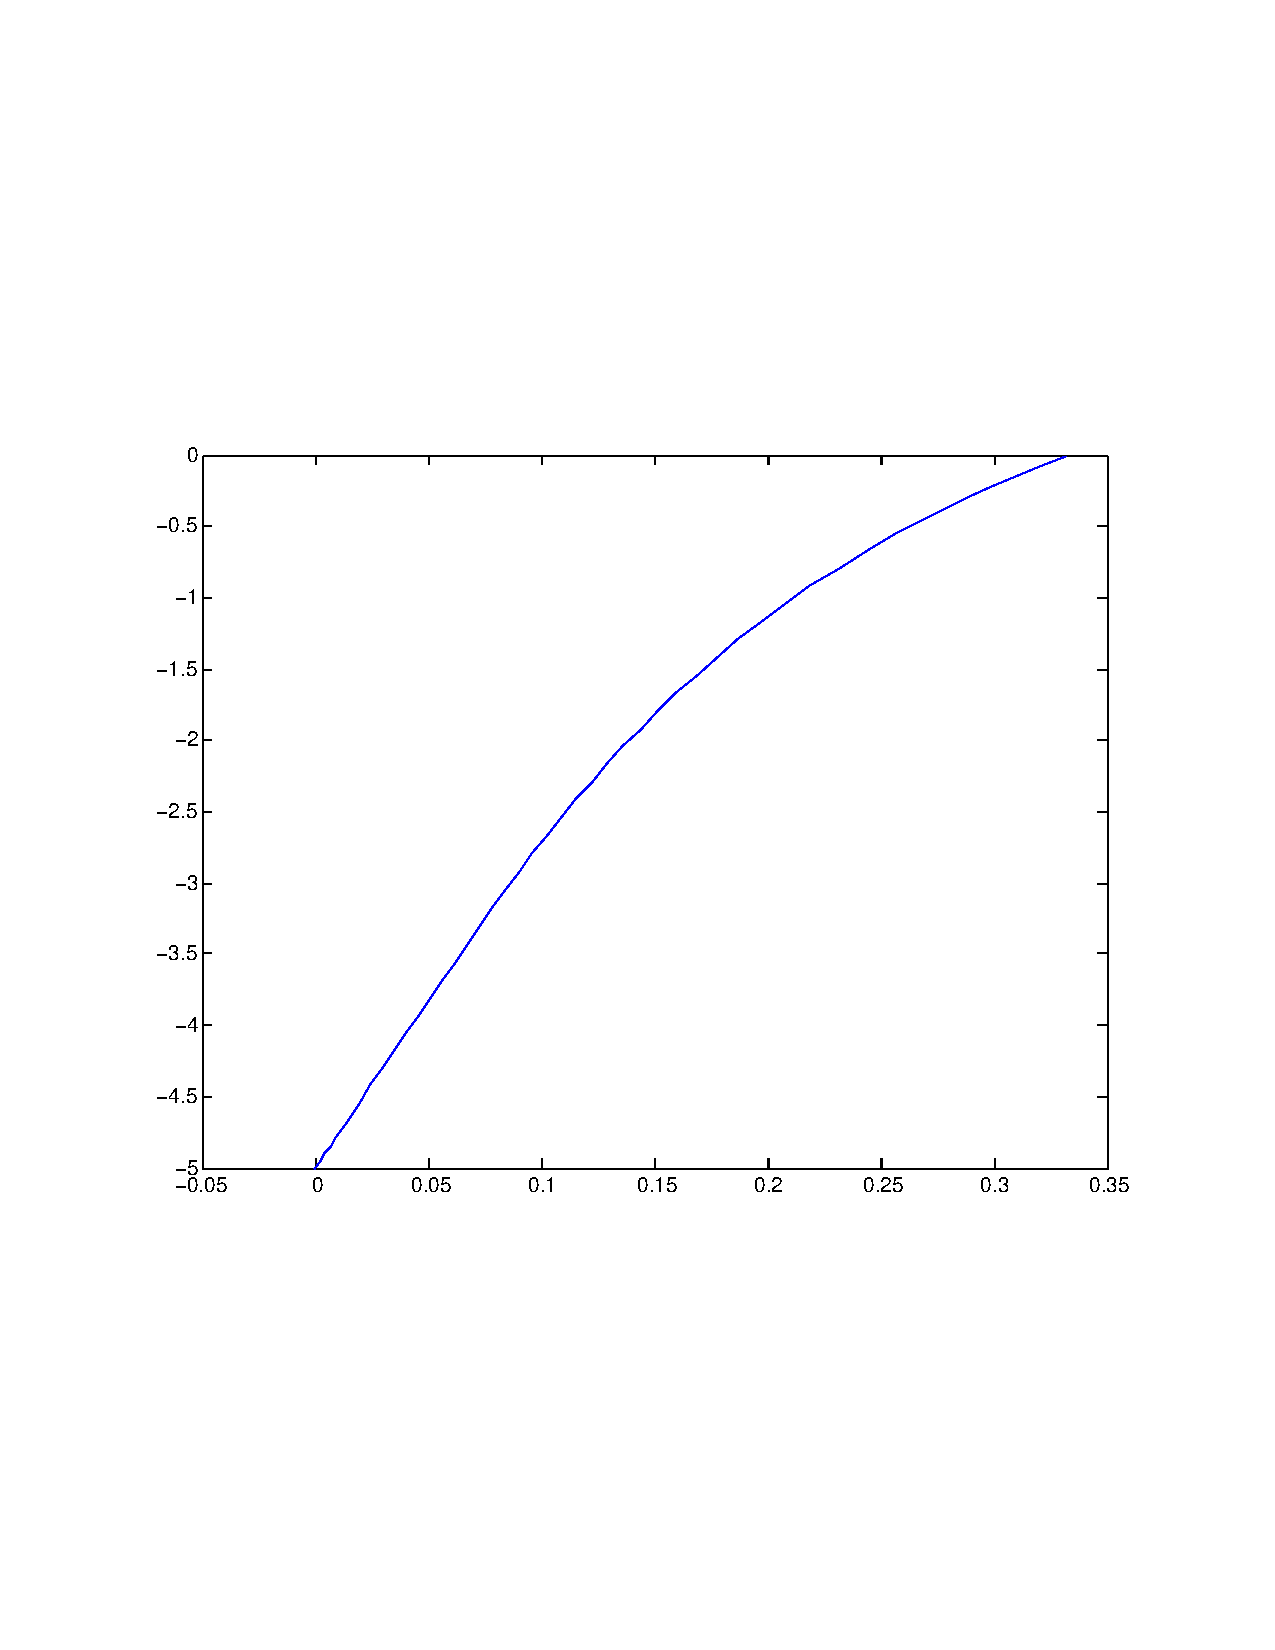
\includegraphics[scale=0.5]{vegetation}
\paragraph{ Profile of velocity inside the vegetation }
\end{document}